\chapter{Preliminaries}
\label{chapter:preliminaries}

This chapter summarizes the preliminary knowledge needed for a high-level understanding of this thesis. It details the concept of Model United Nations and my personal experience with MUN. It also defines the idea of a social network. Then it introduces graph database technologies, focusing on the property graph data model and the Neo4j graph database.

\section{The Model United Nations framework}
\label{section:munframework}

\subsection{Introduction}

The Model United Nations (MUN) framework is an academic simulation of the everyday operation of the United Nations (UN). It is typically an extra-curricular activity materializing as annual, few-day-long conferences organized by students of high schools or universities. Participants welcomed from all over the world take on the roles of assigned nations' UN delegates, forming diplomatic delegations with their peers. There are hundreds of such conferences taking place every year~\cite{mymunconferencelist}. While a medium-size conference has a few hundred participants and another few hundreds of organizers, the current largest Model UN conference — The Hague International Model United Nations (THIMUN) — attracts over 3,200 students from around 200 schools, from more than 100 different countries~\cite{thimunabout}.

Delegates are placed in UN-like committees, where they discuss topics related to international issues and conflicts by the methods of moderated formal debate. The conduct of the debates and the conference is specified in the \emph{Rules of Procedure}, a conference-specific, formal regulation derived from a similar document of the United Nations~\cite{unmunrop}. The result of the debate is a UN-like \emph{resolution}: a formal document expressing the opinion or will of a committee. Resolutions are generally recommendations, but in some cases — like in case of a resolution adopted by the Security Council: the UN body with \textquote{primary responsibility for the maintenance of international peace and security}~\cite{uncharter} — the adopted resolution is legally binding for all member states. Although MUN resolutions of course are never legally binding, larger MUN conferences like THIMUN forward their adopted resolutions to the UN. These forwarded MUN resolutions are occasionally formulated into real-world UN resolutions after further debate and amendments.

The country and committee assignments are known in advance, which enables delegates to perform research and develop their positions before the conference. Students usually build their stances upon the actual standpoints of the countries they represent, but this is not a requirement. Since usually all positions of a given country's diplomatic delegation is assigned to students arriving from the same school, delegates representing the same country can construct complex nationwide strategies across different committees by cooperating with each other in advance.

The larger a conference is, the more possibilities it has regarding the simulation of the actual workings of the UN, or — as the community reinvents itself — even other intergovernmental bodies, like subsidiaries of the European Union. Even though the UN has only 193 member states~\cite{unmembers}, simultaneously simulating the whole operation of the six main organs\footnote{The six main organs of the UN are: the General Assembly with several subsidiary boards, commissions, committees, councils, panels, working groups and others~\cite{gasubsidiaries}; the Security Council; the Economic and Social Council; the Trusteeship Council; the International Court of Justice; and the Secretariat~\cite{unmainorgans}.}, and the Secretariat of the UN requires much more participants.

\subsection{History}

The history of Model United Nations dates back to the early 20\textsuperscript{th} century. The first similar event is believed to have been held in November 1921 by the Oxford International Assembly~\cite{historyofthefirstmun}. It was based on the operation of the League of Nations, the first worldwide intergovernmental organization founded by the Allied powers after the First World War to maintain world peace. Although the League of Nations was formally disbanded in 1946 and its powers were transferred to the United Nations established in 1945, the organization marks an important milestone of intergovernmental cooperation~\cite{leagueofnationsbritannica}.

The first well-documented Model League of Nations conference was organized by the Harvard International Assembly in 1923. It featured the same basic characteristics that modern MUN conferences have: it was organized by an academic institution, had moderated formal debate about international conflicts in committees, and had resolutions adopted as the result of the work conducted during the conference~\cite{historyofthefirstmun}.

The era of Model United Nations started in the 1950s with the establishment of the first high school MUN, Berkeley Model United Nations in 1952, and two other MUNs founded by Harvard University: Harvard Model United Nations in 1953 and Harvard National Model United Nations in 1954. The founding of The Hague International Model United Nations in 1968 led to the global expansion of high school MUN conferences~\cite{top10eventsofmun}. THIMUN was the first MUN in Europe, and is today's largest MUN conference~\cite{thimunabout}. In 1991, the Harvard WorldMUN, a university level MUN rapidly accelerated the spread of university-level MUN. In 2007, the actuation of the BestDelegate.com portal significantly increased the online existence of MUN, providing research and preparatory resources for delegates attending MUN conferences. Founding of MyMUN, an MUN-specific registration and administration system, and MUNPlanet\footnote{At the time of writing this thesis, the website of MUNPlanet~\cite{munplanetwebsite} is not reachable, and its Facebook page~\cite{munplanetfacebook} having more than 150,000 followers received its last update in June 2019.}, an MUN-specific social and knowledge-sharing network furthered the presence of Model United Nations on the Internet~\cite{top10eventsofmun}.

\subsection{MUN in numbers}

I have not found any databases, publications, or studies, which would yield satisfactory statistics about Model United Nations. However, according to several portals, websites and Facebook-pages, we can make assumptions about the worldwide spread of MUN.

\subsubsection{Conferences}

At the time of writing this thesis, MyMUN lists 2,457 conferences from December 2012 until today~\cite{mymunconferencelist}. Calculating with roughly 8 years, and with the broad simplification that there were an equal number of conferences organized every year, there are annually more than 300 conferences worldwide, at least based on solely the data of MyMUN. Considering that MyMUN covers only a small fraction of all MUNs in the world, the number of annual MUN conferences likely goes well into the order of thousands.

\subsubsection{Participants}

MyMUN claims having over 100,000 registered members and over 900,000 yearly visitors~\cite{mymunwebsite}. The Facebook page of MUNPlanet~\cite{munplanetfacebook} has over 150,000 followers. According to a 2007 calculation~\cite{howbigismun}, there are 180,000 MUN participants in the United States only. The BestDelegate.com portal is used by over 750,000 people worldwide~\cite{bestdelegate-about}. Considering the numbers above and MUN's increasing popularity, I would assume that millions of unique students attend Model United Nations conferences every year.

\subsection{Networking within Model United Nations}

MUN conferences offer a number of networking opportunities. First of all, delegates attend committee sessions, where they debate international issues, cooperate in producing resolutions, and leverage simulated international relations along their represented countries' best interests. Therefore the main contact point among them is work: they get to know fellow delegates by observing their leadership, public speaking, and negotiation skills in a competitive field. Committee and lunch breaks enable them to further their acquaintances during the day either professionally or personally.

Professional diplomats attending conferences as guests can also take part in committee sessions as observers, or as actual delegates or chairpersons, but they are more likely to attend the official ceremonies or soirées\footnote{elegant evening party, usually with snacks and drinks}. This way, delegates can interact with professional diplomats without unnecessary formalities of real-world diplomacy. Career diplomats are renowned to have appreciable social skills~\cite{fsicapabilities}, which in this setting helps further mellow the atmosphere, and leads to fruitful conversations between generations.

Besides professional programs like debate sessions and official ceremonies, conferences provide a number of other opportunities for delegates to get acquainted with each other. Events like organized sightseeings and afterwork parties allows building informal bonds alongside professional ones.

Aside from maintaining virtual friendships, members of the MUN community often harmonize their conference participations to meet with their foreign acquaintances. Since there is no suitable networking platform for this scenario, participants from different countries usually keep connected and communicate via general social networks, like Facebook. Due to the lack of Facebook's MUN-specific capabilities, a large part of the networking effect is lost, as delegates are not given automated suggestions on which conferences to attend based either on their circle of friends, or on their previous Model UN experience.

\subsection{Administration of a Model United Nations conference}

The general administration of a conference can be divided to two distinct parts. The \emph{professional division} involves administrative tasks related to the Model United Nations framework itself: composing the discussed topics, assigning countries and committees to members of delegations, conducting the actual debates and formal ceremonies, and other features associated with diplomacy. The professional division encompasses everything inside the simulation, where the participants are in their diplomatic roles. The \emph{organizational division} covers the real-world event outside the simulation: travel and hotel arrangements, meals, conference accessories, merchandise, entertainment, among others. According to my personal organizational experience to be detailed in \Cref{section:personalexperience}, the two divisions are separate responsibilities requiring completely different experience, and thus are best to be kept as isolated as possible.

Similarly to the United Nations, the chief administrative officer of an MUN conference is usually the \emph{Secretary-General}, responsible for organizing, administering and conducting the conference. In case of the aforementioned two-division administrative approach, the Secretary-General is responsible only for the professional division of the conference, and reports to the \emph{Conference Manager} or \emph{Project Manager}, who leads the organizational division, and is responsible for the entire conference. Henceforth I refer to the organizational and professional divisions together as management.

In the following sections I detail the procedure of organizing a medium-size, high school-level MUN conference with the two-division administrative approach, broken down to distinct, preemptive phases. Most of the following is based on my personal experience, but it also contains parts I learned from event planners or other Model United Nations conference organizers.

\subsubsection{Preliminary arrangements}

Once the management of the previous year's session agreed upon their successors, the new management starts negotiations with the headmaster of the organizing school. They settle the dates for the conference, discuss necessary resources the school can provide, and start or continue securing external locations\footnote{External locations are often needed to be secured years in advance.} for larger conference ceremonies involving all participants, which the school usually cannot host.

After the initial negotiations, the management announces the conference's subsequent session in the host school with its date and vacancies in the organizational structure, and starts coordinating interviews with eventual applicants wishing to take part in organizing the conference.

\subsubsection{Participants' application to the conference}

After the professional division agreed on the UN bodies to be simulated, they publish preliminary committee assignments with high-level topics on the conference's website or Facebook page. As the management opens the application for participants, delegations and individual delegates apply to the conference specifying their preferences of country and committee assignments. Since high school students rarely travel abroad alone, a delegation is usually accompanied by a couple of teachers of the applicants' school. The accompanying teachers are recorded into the registration system as well as the students.

The application procedure comes with significant paperwork. The management consisting of junior members usually lack the experience and resources for efficiently and securely processing sensitive personal information\footnote{Registration data usually includes the applicant's name, birthdate, email address, phone number, and home address. It is also common to require the applicant's social security number or even the serial number of their passport for speeding up any immigration-related checks and administration.} of hundreds or thousands of applicants, and a school's IT division cannot be expected to be prepared for developing a suitable system either. Thus it is common that the registration is implemented with a simple online form populating insecure spreadsheets, or a primitive in-house application often making data management only more complex. Ready-to-use software like MyMUN are often not customizable enough to be useful for conferences generally requiring somewhat tailored solutions, which leads to the usage of multiple different applications. This can cause more pain than gain by requiring manual data maintenance in unintegrated systems.

\subsubsection{Accepting or rejecting applications \& finalizing country and committee assignments}

Following the closure of the application procedure, the management decides about the acceptance or rejection of prospective participants. As applicants usually register as part of their school's delegation consisting of multiple delegates, it is common that the application of an entire delegation gets accepted or rejected together.

Whether to accept a delegation's application to the conference is decided by considering various factors: these can include the delegation's level of expertise — often with regards to the reputation of previously attended conferences —, the ability of fulfilling their preferences of represented countries provided at registration, and aspects of diversity, among others. In case of more mature conferences, committees are often classified by their members' expected level of MUN experience. A beginner delegate taking a seat in an expert-level committee is inexpedient, as it sets back the efficiency of the debate, or vice versa, it prevents the delegate from staying on their learning curve.

Accepting delegations happens in the interest of filling committee seats — predefined seats of countries represented in committees — in the best possible combination with regards to expertise, personal preference, diversity, and the prospective efficiency of the committee's work. Creating the final assignments of delegations and country-committee pairs can be challenging if done manually, considering the volume of input data, and the factors needed to be taken into account. Most conferences do the entire assignment process by hand, in spreadsheets, along a malleable set of priorities. This usually means playing with the synthesis of the committees until all delegations desired by the management can be offered a place to the conference close to their preferences.

This process can be automated, if the management composes a definitive set of priorities on how to assign already fixed committee seats — country-committee pairs — to the applied delegates as individuals. The problem of creating the assignments with the aforementioned conditions is a fundamental problem of combinatorial optimization: it is called \emph{maximum weighted bipartite matching} or \emph{assignment problem}~\cite{ropi}. Mathematically speaking, we are looking for the maximum-size matching in a weighted bipartite graph, where the sum of the edges' weight is maximal. One part of the graph is the set of applicants, and the other part is the set of committee seats. The edges between parts represent possible assignments, and their weights are \textquote{goodness} values based on assignment priorities composed by the management. Since this approach does not cover the possible requirement of all delegates from the same school needing to represent the same country, it is not always satisfactory.

If same-school students need to represent the same country, the process can still be automated with maximum weighted bipartite matching, but with an additional constraint: the management must restrict the application to fixed-size delegations. In this case, a participant school's fixed-size delegation applies to the conference as a whole, specifying their preferences from the set of same-size delegations of represented countries on the conference. This way, the bipartite graph's two parts consist of school delegations applied and country delegations represented on the conference. An edge between the two parts means that the two kinds of delegation are of the same size, so they can be assigned to each other. The weight of an edge is the same \textquote{goodness} value based on assignment priorities composed by the management. This approach needs a second application step: after applied school delegations were assigned country delegations represented on the conference, the applicants of the delegations need to distribute the assigned committee seats among themselves.

\subsubsection{Payment}

The participation fees are collected after the registration, generally in multiple parts. International bank transfers executed by students and teachers usually renders the work of the conference's accounting department challenging, as it is often difficult to identify which delegation made which payment. Due to the general lack of integrated payment solutions in the MUN scene, conferences often face a heavy burden of financial paperwork.

A conference management system with integrated payment processing and accounting features could solve these organizational problems. It would also provide a cleaner experience to the participants: they could pay instantly and individually, without the troubles of needing to transfer the money in groups, as whole delegations.

\subsubsection{Travel, hotel, meal and other arrangements for participants}

With the closure of the acceptance and the assignments procedure, the final list of students and their accompanying teachers attending the conference becomes available, and the management can start working on participants' personalized experience. Though habits differ, most conferences offer various convenience services for additional fees, such as transport within the city, accomodation, meal arrangements, and tailored sightseeing or other entertainment programs. This causes lots of additional paperwork with regards to the delegation's arrival and departure dates, hotel or other kinds of accomodation preferences, and several kinds of meal allergies and eating habits\footnote{Since participants arrive from all around the world, conferences generally offer multiple types of menus respecting various cultures and allergies.}.

Similarly to the registration, most of the organizational paperwork in connection with convenience services is done manually. A capable software system possessing all information of a delegation's precise schedule, as well as their hotel, meal and entertainment preferences, could automate all this paperwork. This would allow the management to focus on the quality of the provided services instead of administration. Also, it would open additional financial possibilities. Following preliminary arrangements between the conference management and hotels or other service providers, the applicants could purchase their necessities by selecting them from a list of integrated services during the application procedure. This would endorse further financial cooperation between parties — the conference, the company providing conference management software, and the service providers —, while providing a simple, one-step payment flow for the participants.

\subsubsection{Personalized conference accessories}

MUN conferences formally require participant students, teachers, and all other conference personnel to possess various personalized items. Every person — participants, guests, organizers, staff — should wear an official, conference-issued badge during all events of the conference. The badge usually describes the person's name and title — either a diplomatic one within the simulation in case of participants or guests, or an organizational one in case of organizers or members of staff. Participant delegates, chairpersons, teachers, guests and everyone else attending committee sessions should have official, conference-issued placards in front of them, describing their represented country or position within the committee. Placards are used for voting in larger committees, as well as for identifying delegates from the distance.

Producing hundreds or thousands of personalized items without experience and proper tools can be time-consuming. Management teams generally possess neither the experience nor the tools, which leads to hours or days of manual work of creating personalized elements, one by one. Besides being error-prone, this process consumes valuable organizational resources. A capable software possessing all necessary information about participants and organizers could automate this manual work.

\subsubsection{Conducting the conference}

Following a half-year or longer period consisting of planning and preparation only, conducting the conference itself is usually not a real challenge. Administratively, the management needs to record whether incoming delegations signed in, and received their conference packages, but from the opening ceremony through the committee sessions and parties to the closing ceremony, the conference generally goes by itself, being already scheduled well.

\subsubsection{Processing and storing resolutions and conference data}

Few MUN conferences pay attention to the collection and storage of conference data. As management teams usually lack the resources and experience for keeping digital or paper-based documents, produced resolutions and other conference data is generally not preserved. A capable conference management system could offer solutions for this: with online resolution editing and automated video recording features, the management would not even need to collect conference data, because all of it would immediately be saved in the conference management software's permanent online database.

\subsection{Personal experience: Budapest International Model United Nations}
\label{section:personalexperience}

The previous section's points are mostly based on my personal organizational experience regarding Model United Nations. My former high school, József Eötvös Secondary Grammar School, located in the 5\textsuperscript{th} district of Budapest, first organized \emph{Budapest International Model United Nations (BIMUN)} in April 2011\footnote{The school has organized BIMUN conferences every year since then. Unfortunately, the tenth anniversary session of BIMUN, which would have been held this year, got cancelled due to the COVID-19 pandemic.}. BIMUN was among the first large-scale international MUN conferences in Hungary~\cite{bimunhistory}. Previously I had attended several foreign MUN conferences, and I was looking forward to taking part in the organizational process of an international conference welcoming hundreds of students and diplomatic guests. Over the course of 6 years, I fulfilled several positions: I was a photographer, team lead, deputy Secretary-General, and part of the chief management as an executive advisor.

\section{Social networks}

\subsection{Introduction}

The term social network is used in social sciences, denoting a network of linked individuals or organizations, connected by social relations and interactions~\cite{Borgatti892}. This thesis focuses on another aspect of social networks: online software providing networking, information sharing and messaging features for participating individuals or organizations. The two interpretations are related: users of a social network software form a social network in the scientific sense, and a social network can be loaded into a social network software for analysing patterns, or simply for facilitating interactions among social actors. Analysing social networks can be useful in various fields, including organizational studies and information sciences, and also in diplomacy~\cite{networkdiplomacy}.

\subsection{Connection with graph theory}

Since social networks essentially are connected entities, an obvious choice for modeling such networks is using graphs, where vertices are individuals or organizations, and edges are connections or interactions between them. This way networks are easier to visualize and understand~\cite{socialnetworkvisualization}, and graph algorithms are useful for various kinds of analyses~\cite{socialnetworkanalysis}. By using different kinds of edges in the same graph, several kinds of connections can be represented within the same entity set, allowing to build a multi-dimensional model of the network. This can lead to deeper insight into network structure.

\subsection{Social networking services}

In this thesis I consider social networking services as social networks with associated features the network members can utilize, offered as mass-available services on the Internet. Besides the core networking activity of building relationships within the network itself, associated features can include messaging, information sharing, and collaborational functionality, among others. Usually the goal of a social network is to provide the possibility of interaction among participants, beyond actual in-person interactions. This enables individuals to connect with others regardless of physical distance.

Social networks can be categorized into four main types~\cite{thelwall2009}, but with regards to the focus of this thesis, I divide the set of social networks into two parts.

\begin{itemize}
\item \emph{Generic social networks} have no special characteristics or determined target audience: they offer a set of generic features for people to build and maintain virtual relationships with or without personal acquaintance.
\item \emph{Domain-specific social networks} have a determined target audience: they offer specialized features for members of the target audience in line with specific goals of usage in a given domain.
\end{itemize}

Real-world examples for generic social networks include Facebook~\cite{aboutfacebook}, Twitter~\cite{abouttwitter}, and Instagram~\cite{aboutinstagram}. Facebook is the biggest social networking service in the world, having approximately 2.6 billion monthly active users~\cite{facebook2020q1report}. It has several kinds of features for sharing ideas, photos, live or recorded videos, connecting with friends, and informing others in various ways. It also offers basic event-handling capabilities for facilitating in-person social interactions. Facebook's business model is based on targeted, personalized advertisement: it offers free features for users, who receive ads in their newsfeed and on other interfaces~\cite{fb-business-model}. The platform has been continuously learning user preferences, and personalizes ads according to the user's assumed needs. Facebook's financial income is mostly based on the fees paid by businesses for publishing and targeting their advertisements in various applications of the social networking platform.

Twitter is a social network that gained popularity by providing microblogging features. Users can publish short \textquote{tweets}: posts with at most 280 characters\footnote{Until 2017 November, the maximum length of a tweet was 140 characters~\cite{twitter-doubling-character-limit}.}. It is asymmetric, meaning users can follow other users instead of needing to get virtually acquainted — although for private profiles, users need to be explicitly granted access. Twitter has approximately 166 million daily active users~\cite{twitter2020q1report}, and builds its revenue upon advertising and data licensing~\cite{twitter-business-model}.

Instagram is a social network primarily used for sharing photographs capturing important moments. Despite the fact that it is mainly used for image sharing, Instagram can still be regarded as a generic social network, because it is not to be interpreted within a specific domain, and has no determined target audience. Similarly to Twitter, it is asymmetric, but also has private profiles. Instagram was acquired by Facebook in 2012~\cite{facebookacquiresinstagram}, and shares the same basic characteristics regarding its business model: users receive sponsored posts and stories as personalized advertisements.

Diplomatiq is a domain-specific social network. Its domain is diplomacy, its target audience is the set of junior and senior diplomats and other people working in diplomacy, and its specialized features — currently a very basic set of functionalities — include organizing MUN conferences. Broadening the capabilities of Diplomatiq will expectedly not alter its domain-specificity. Further domain-specific social networks are mentioned in \Cref{chapter:relatedwork}.

\section{Graph database technologies}

Graphs are mathematically defined data structures being broadly used in several fields of computer science. Recent technologies and implementations made possible for developers to easily embed graph data models into their applications. There are numerous real-world scenarios which can be represented more efficiently as graphs (\emph{nodes} connected to each other by \emph{edges}), than with the traditional, relational approach.

Graph databases are NoSQL databases, which store data in graphs instead of the traditional, table-based approach\footnote{The underlying data storage methods vary. There are graph databases which store graph data in relational tables, introducing another layer of abstraction between the stored physical data and the database.}. In graph databases, a relationship represented as an edge in the graph is a \textquote{first-class} entity, and has the same basic storage characteristics as a node. Relationships are directly linked to entities, and therefore entities are directly linked to each other via relationships. This allows the querying of related entities to be fast, since the process does not involve lookups.

\subsection{The property graph data model}

It is common to define graphs as a set of objects, in which some object pairs are connected to each other. In this model, an object is called \emph{vertex} or \emph{node} or \emph{point}, and a connection between two \emph{vertices} is called \emph{edge} or \emph{relation}. Connections can be detailed further by specifying their directionality, also they can be \emph{labeled} to define them even more. Similarly labeling vertices leads to the model of \emph{typed graphs}. If we assign properties to the nodes or relations, we get the model of \emph{property graphs}. Properties, as shown in \Cref{fig:property-graph}, are usually key-value pairs in the format of \lstinline{key = `value'}. Generally, keys are strings, and values represent common data types like string, integer, float, etc.

\begin{figure}[!htb]
    \centering
    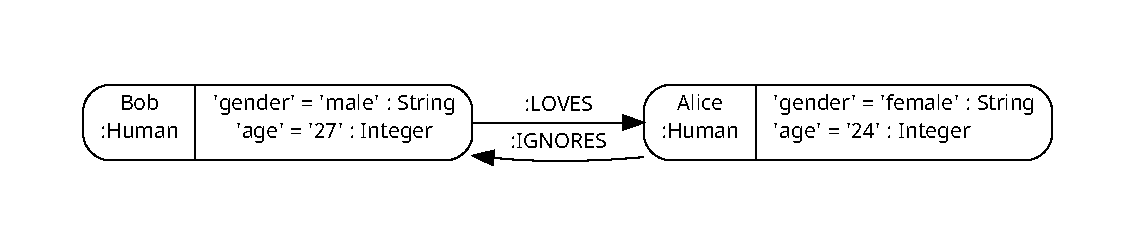
\includegraphics[width=\textwidth, trim=12mm 12mm 12mm 12mm,clip]{figures/property-graph.pdf}
    \caption{Two persons' relationship modeled with a property graph}
    \label{fig:property-graph}
\end{figure}

\subsection{Neo4j}

Among a handful of graph database vendors~\cite{graph-dbs}, Neo Technology's Neo4j is the most popular one~\cite{graph-dbs-raking}. It features full ACID-compliance upon a pure graph data model, contrary to other vendors' multi-model approaches. Besides Neo Technology, Neo4j is backed by the open-source community as well~\cite{neo4j-github}. There are two variants: \emph{Community Edition} and \emph{Enterprise Edition} with an extended feature set~\cite{neo4j-licensing}. Neo4j also offers a program tailored to startup companies~\cite{neo4j-startup-program}. With the help of this startup program, companies can build their applications on the Enterprise Edition of the Neo4j platform, free of charge\footnote{Certain limitations apply: the company must have at most 50 employees and at most \$3 million annual revenue, among others~\cite{neo4j-startup-program}.}.

\subsection{Cypher}

Cypher is a query language developed especially for graph databases by Neo Technology~\cite{neo4j-cypher}. \Cref{fig:cypher-intro} shows that the language uses a sort of ASCII-art to represent nodes and relationships: nodes are in parentheses, relationships are in brackets surrounded by relationship direction information.

\begin{figure}[!htb]
    \centering
    \lstinline{(Bob)-[:LOVES]->(Alice)}
    \caption{A basic Cypher example}
    \label{fig:cypher-intro}
\end{figure}

Cypher syntax is elegant and expressive, thus very readable. Besides using it to represent nodes and relationships, we can utilize it to access the Neo4j's indexing capabilities and stored procedures as well. Even complex pattern-matching conditions can be expressed easily and intuitively in Cypher. Although today's modern application development frameworks — adopting increasingly capable data mapping solutions — make it less and less necessary to directly interact with databases, complex queries can still involve composing database commands manually. Therefore the expressiveness and ease of use of a database query language still remains essential.
